\documentclass[review,3p]{elsarticle}

\usepackage{lineno}       
\modulolinenumbers[5]
\usepackage{subcaption}             % used in subtable

\usepackage{graphicx}

\usepackage{amsmath, amsfonts, amsthm}            % for subequations

\usepackage{mathtools, amssymb}          % for \leqslant
\newcommand{\ddn}[2]{\frac{\mathrm{d}}{\mathrm{d}#1}#2}
\newcommand{\ddt}{\frac{\mathrm{d}}{\mathrm{d}t}}

\usepackage{upgreek}
\usepackage[dvipsnames]{xcolor}
\usepackage{soul}
\usepackage{multirow}

\usepackage{array}
\newcolumntype{C}[1]{>{\centering\let\newline\\\arraybackslash\hspace{0pt}}m{#1}} 
\newcolumntype{L}[1]{>{\raggedright\let\newline\\\arraybackslash\hspace{0pt}}m{#1}} 
\newcolumntype{R}[1]{>{\raggedleft\let\newline\\\arraybackslash\hspace{0pt}}m{#1}} 

\usepackage{booktabs}       % http://ctan.org/pkg/booktabs

\newcommand{\tabitem}{~~\llap{\textbullet}~~}           % for items inside a table
\usepackage{makecell}       % used inside a table
\usepackage{pbox}           % for weak form 3
\usepackage{empheq}
\newcommand*\widefbox[1]{\fbox{\hspace{2em}#1\hspace{2em}}}


\usepackage{colortbl}
\usepackage{esvect}
\usepackage{spreadtab}
\usepackage{numprint}
\usepackage{xstring}
\renewcommand*{\thefootnote}{\fnsymbol{footnote}}
\usepackage[symbol]{footmisc}

\usepackage{siunitx}

\makeatletter       % for rom in deal.ii symbol
\newcommand*{\rom}[1]{\expandafter\@slowromancap\romannumeral #1@}
\makeatother

\usepackage{enumitem}

\usepackage{hyperref}               


\usepackage{cleveref}
\crefformat{section}{\S#2#1#3} % see manual of cleveref, section 8.2.1
\crefformat{subsection}{\S#2#1#3}
\crefformat{subsubsection}{\S#2#1#3}

\captionsetup[figure]{labelfont={bf},name={Fig.},labelsep=period}
\captionsetup[table]{labelfont={bf},name={Table},labelsep=space,justification=justified,singlelinecheck=false}      % the last two commands for left-align the caption

\usepackage[labelformat=simple]{subcaption}	        	% order of subfigure with brackets
\renewcommand\thesubfigure{(\alph{subfigure})}
\renewcommand\thesubtable{(\alph{subtable})}


\usepackage{wrapfig}
\usepackage{lipsum}

\usepackage{pgfplots}       % for tikzpicture
\pgfplotsset{compat=1.7}

\pdfsuppresswarningpagegroup=1      % eliminate warning 'multiple pdfs with page group included in a single page'

\usepackage[ruled,linesnumbered]{algorithm2e}		% for algorithm

\begin{document}

\begin{frontmatter}

\title{Balancing truncation and round-off errors in practical FEM: one-dimensional analysis}

 \author[1]{Jie Liu\corref{cor1}}
 \ead{j.liu-5@tudelft.nl}
 \author[1]{Matthias Möller}
 \ead{m.moller@tudelft.nl}
 \author[1]{Henk M. Schuttelaars}
 \ead{h.m.schuttelaars@tudelft.nl}
 
 \address[1]{Delft Institute of Applied Mathematics\\ Delft University of Technology\\ Van Mourik Broekmanweg 6, 2628 XE Delft, The Netherlands}
\cortext[cor1]{Corresponding author}

\begin{abstract}
In finite element methods (FEMs), the solution accuracy cannot be improved indefinitely because of the limited computer precision. We propose an innovative method to find the highest attainable accuracy based on the round-off error for the one-dimensional second-order ordinal differential equations. This method uses a formula to save several computations on fine grids. The application of our method to a complex-valued Helmholtz equation in space shows that the highest attainable accuracy can be accurately predicted, while the CPU time required is much less. 
\end{abstract}


\begin{keyword}
Finite Element Method (FEM), differential equation, round-off error, highest attainable accuracy, estimation.
\end{keyword}

\end{frontmatter}

\section{Introduction}

Many problems in engineering sciences and industry are modelled mathematically by initial-boundary value problems comprising systems of coupled, nonlinear partial and/or ordinary differential equations. These problems often consider complex geometries, with initial and/or boundary conditions that depend on measured data \cite{Kumar2016}. 
In some applications, not only the solution, but also its derivatives are of interest \cite{Kumar2016,carey1982derivative}.
For many problems of practical interest, analytical or semi-analytical solutions are not available, and hence one has to resort to numerical solution methods, such as the finite difference, finite volume, and finite element methods. The latter will be adopted throughout this paper and applied to one-dimensional boundary value problems.

The accuracy of the numerically obtained solution is influenced by many sources of errors \cite{ferziger2012computational}: firstly, errors in the set-up of the model, such as the simplification of the domain and governing equations and the approximation of the initial and boundary conditions; next, truncation errors due to the discretization of the computational domain and use of basis functions for the function spaces defined on it; then, round-off errors due to the adoption of finite-precision computer arithmetics, rather than exact arithmetics; finally, iteration error resulting from the artificially controlled tolerance of iterative solvers. We focus on the error led by the truncation and round-off if not stated otherwise.

One tacitly assumes that the two types of errors are well-balanced. That is, the round-off error is often ignored based on the argument that it will be `sufficiently small' if just IEEE-754 double-precision floating-point arithmetics are adopted.
However, with the popularity of high-order approximations, the round-off error is likely to play a role with only a small number of degrees of freedom (DoFs). Despite this alarming observation, to the authors’ best knowledge, only very few publications address the impact of accumulated round-off errors on the overall accuracy of the final solution or take them into account explicitly in the error-estimation procedure {\cite{ling1984numerical,mou2017example,ainsworth1992procedure,alvarez2012round}}.
The general rule of thumb is still to perform as many $h$-refinements as possible considering the available computer hardware.

The aim of this paper is to systematically analyze the influence of round-off on the error for the solution and its first and second derivative, and propose a practical approach for obtaining the highest attainable accuracy determined by the round-off error (${E}_{\rm {min}}$).
The scope is restricted to one-dimensional second-order model problems, for which the existence of the second derivative of the solution is guaranteed in the weak sense. Moreover, we consider both the standard finite element method (FEM) and mixed FEM\cite{boffi2013mixed}.

The paper is organized as follows. The model problem, finite element formulation and numerical implementation are described in Section \ref{section_model_problem_FEM_formulation_numerical_implementation}. The general behavior of the error and the approach to predict ${E}_{\rm {min}}$ are discussed in Section \ref{approach_finding_optimal_number_of_DoFs}. The constants used in the approach are determined in Section \ref{section_error_constants}, followed by an algorithm for realizing the approach and its application in Section \ref{section_algorithm_application}. The conclusions are drawn in Section \ref{paragraph on conclusion}.

\section{Model problem, finite element formulation and numerical implementation}	\label{section_model_problem_FEM_formulation_numerical_implementation}

\subsection{Model problem}

Consider the following one-dimensional second-order differential equation:
\begin{equation}
  -\left(d(x) u_x \right)_x + r(x)u(x) = f(x),\qquad x \in I = (0,1),	\label{1d_second_order_differential_equation}
\end{equation}
with $u$ denoting the unknown variable, which can either be real or complex, $f(x) \in L^2 (I)$ a prescribed right-hand side, and $d(x)$ and $r(x)$ continuous coefficient functions.
By choosing $d(x)=1$ and $r(x)=0$, Eq. (\ref{1d_second_order_differential_equation}) reduces to the Poisson equation; for $d(x)>0$ and not constant, the diffusion equation is found when $r(x)=0$, and the Helmholtz equation is found when $r(x) \neq 0$. 
The boundary conditions are $u(x)=g(x)$ on $\Gamma_D$ and $d(x)u_x=h(x)$ on $\Gamma_N$. Here, $\Gamma_D$ and $\Gamma_N$ are the boundaries where Dirichlet and Neumann boundary conditions are imposed, respectively.

\subsection{Finite element formulation} 	\label{FE formulation}

For convenience, we introduce the two inner products:
 \begin{subequations}
  \begin{align}
   (f_1(x), \,f_2(x) ) &= \int _I f_1(x) f_2(x) \, dx,	\\
   (g_1(x), \,g_2(x) )_{\Gamma} &= g_1(x_0) g_2(x_0).
  \end{align}
 \end{subequations}
where $f_1(x)$, $f_2(x)$, $g_1(x)$ and $g_2(x)$ are continuous functions defined on the unit interval $I$, $\Gamma$ denotes the boundary of $I$, and $x_0$ the coordinate on $\Gamma$.

\subsubsection{The standard FEM}

The weak form of Eq. (\ref{1d_second_order_differential_equation}) is derived in \ref{derivation_weak_form_SM}. Imposing the Dirichlet boundary conditions strongly, the weak form reads:
\begin{equation}
\centering
\boxed{ 
\begin{aligned}
&\text{Weak~form}~ 1 ~~~~~~~~~\\
&\text{Find $u \in H _D^1 (I)$ such that:} \\
&({ \eta} _{ x }, \, du _{ x }  ) + (\eta, \, ru) = (\eta, \, f ) + (\eta, \, hn)_{\Gamma _N} \qquad \forall \eta \in H _{D0}^1 (I),\\
&\text{with} \\
&~~~~~~~~~~~~~H_{D} ^1 (I) = \{t \; | \; t \in H^1 (I), \; t = g \text{ on } \Gamma _D \},  \\
&~~~~~~~~~~~~H_{D0} ^1 (I) = \{t \; | \; t \in H^1 (I), \; t = 0 \text{ on } \Gamma _D\},\\
&\text{where } {n} \text{ is 1 at $x=1$, and $-1$ at $x=0$.}
\end{aligned}		\label{1D_general_SM_weak_form_Diri_strong} 
}
\end{equation}
Imposing the Dirichlet boundary conditions in the weak sense\cite{freund1995weakly}, the weak form reads:
\begin{equation}
\centering
\boxed{
\begin{aligned}
&\text{Weak~form}~ 2 ~~~~~~~~~\\
&\text{Find } u \in H ^1 (I) \text{ such that:}\\
& ( { \eta} _{ x }, \, du_x) + (\eta, \, ru) - (\eta, \, du_x n )_{\Gamma _D} + (\eta _x, \, u n )_{\Gamma _D} - (\eta, \, \rho u n )_{\Gamma _D} \\ 
&= (\eta, \, f ) + (\eta, \, h n )_{\Gamma _N} + (\eta _x, \, g n )_{\Gamma _D} - (\eta, \, \rho g n )_{\Gamma _D} \qquad \forall \eta \in H ^1 (I), \\
&\text{where } \rho \text{ is a } \text{{positive}} \text{ value that serves as the penalty parameter}.
\end{aligned}	\label{1D_general_SM_weak_form_Diri_weak}
}
\end{equation}

\noindent Note that, the terms in the right-hand sides of Eqs. (\ref{1D_general_SM_weak_form_Diri_strong})--(\ref{1D_general_SM_weak_form_Diri_weak}) consist of information of Neumann boundary conditions which vanish if they are not prescribed. 

We approximate $u$ by a linear combination of a finite number of basis functions:

\begin{equation}
 u \approx u_h = \sum _ {i=1} ^{m} u _{i} \varphi _{i}. \label{General_SM_u_approx}%
\end{equation}
Here, $m$ is the number of DoFs ($N_h$), $\varphi _{i}$ are $C^0$-continuous Lagrange basis functions supported by Gauss-Lobatto points and $u_i$ are the values of $u_h$ at the DoFs. The resulting system of equations reads
\begin{equation}
 A {U} = F,				\label{matrix equation std FEM}
\end{equation}
where $A$ is the stiffness matrix, $F$ the right-hand side and $U$ the discretized $u$.

\subsubsection{The mixed FEM}
Derived in \ref{derivation_weak_form_MM}, the weak form of Eq. (\ref{1d_second_order_differential_equation}) using the mixed FEM is given by:
\begin{subequations}
\begin{empheq}[box=\fbox]{align}
&\text{Weak~form}~ 3 ~~~~~~~~~\notag\\
&\text{Find $v \in H_{N}^1 (I)$ and $u \in L ^2 (I)$ such that:}	\notag\\
& ~~~~~~~\;(w, \, d^{-1}v) - (w_x, \,  u ) = -(w, \, g n)_{\Gamma_D} \qquad \forall w \in H_{N0}^1 (I), \label{1D_General_MM_weak_1}\\ 
& ~~~~~~~~~- (q, \, v_x) - (q, \, ru) = -(q, \, f) \qquad \forall q \in L ^2 (I), \label{1D_General_MM_weak_2}	\\
&    \text{with}\notag\\
& ~~~~~~~~~~~~~~~ H_{N} ^1 (I) = \{t \; | \; t \in H^1 (I), \; t = -h \text{ on } \Gamma _N \},  \notag\\
& ~~~~~~~~~~~~~\, H_{N0} ^1 (I) = \{t \; | \; t \in H^1 (I), \; t = 0 \text{ on } \Gamma _N\}.	\notag 
\end{empheq}
\label{1D_General_MM_weak_2in1}%
\end{subequations}
Next, we approximate $v$ and $u$ by a linear combination of a finite number of basis functions:
\begin{subequations}
 \begin{align}
 v \approx v _h &= \sum _ {i=1} ^{n} v _{i} \varphi _{i},     \label{General_MM_var_approx1}  \\[3ex]
 u \approx u _h &= \sum\limits _ {j=1} ^{p} u _{cj} \psi _{j} \text{ in cell }c,  \label{General_MM_var_approx2}
\end{align}	\label{General_MM_var_approx}%
\end{subequations}
where $n$ is the number of DoFs for $v_h$, $\varphi _{i}$ are of the same type of basis functions used in Eq. (\ref{General_SM_u_approx}), and $v_i$ are the values of $v_h$ at the DoFs; $p$ is the number of DoFs of $u_h$ in each cell, $\psi _{j}$ are discontinuous Lagrange basis functions, and $u_{c,j}$ are the values of $u_h$ at the DoFs. 
Finally, the resulting coupled linear system of equations that has to be solved reads:
\begin{equation}
 \left[ \begin{array}{cc} M & B  \\ B^\top & 0 \end{array}\right] \left[ \begin{array}{cc} {V} \\ {U} \end{array}\right] =\left[ \begin{array}{cc} G \\ H \end{array}\right], \label{matrix equation mix FEM}
\end{equation}
where the mass matrix $M$, discrete gradient operator $B$, and its transpose, the discrete divergence operator $B^\top$, comprise the left-hand side; $G$ and $H$ are the components of the right-hand side; $V$ and $U$ are the discretized $v$ and $u$.

\subsection{Numerical implementation}

All results are computed in IEEE-754 double precision \cite{zuras2008ieee} using the deal.\rom{2} finite element code \cite{alzetta2018deal}.

\subsubsection{Solution technique}

The computational mesh is obtained by globally refining a single element that covers the interval $I$, and the Dirichlet boundary conditions are imposed strongly unless stated otherwise.
To compute the occurring integrals, sufficiently accurate Gaussian quadrature formulas are used. 
Furthermore, to solve the system of equations, the UMFPACK solver \cite{davis2004algorithm} is used with priority. Last but not least, the derivatives of the numerical solution are computed in the classical finite element manner, e.g. $u_{h,x}=\sum\limits _{i=1}^m u_i\varphi_{i,x}$ yields an approximation to $u_x$ using standard FEM. 

\subsubsection{Error estimation}

For the numerical results $var_h$ of the variable $var$, the error measured in the $L_2$ norm is used. It is defined as
\begin{subequations}	\label{formula_abs_error}
\begin{align}		\label{formula_abs_error_analytical}
 E_{h} &= {\|var_{h}- {var}_{\rm exc}\|_{2}}
\end{align}
when the exact approximation ${var}_{\rm exc}$ is available, or \cite{Runborg2012VerifyingNC}
\begin{align}		\label{formula_abs_error_numerical}
 {\widetilde {E_{h}}} &= {\|var_{h}- {var}_{h/2}\|_{2}}
\end{align}
otherwise,
\end{subequations}
where $var_{h/2}$ is the numerical solution computed on a mesh of grid size $h/2$. 
Furthermore, we compute the order of convergence $Q$ or $\widetilde{Q}$ from either $\log _2 \left( \frac{E_{h}}{E_{h/2}} \right)$ or $\log _2 \left( \frac{\widetilde {E_{h}}}{\widetilde {E_{h/2}}} \right)$, for which the theoretical value is one order higher than the approximation order\cite{gockenbach2006understanding}.


\section{Approach to finding the optimal number of DoFs}                 \label{approach_finding_optimal_number_of_DoFs}


\subsection{Theoretical evolution of the error}

The conceptual sketch of $E_h$ against $N_h$ in the log-log axes can be found in Fig.~\ref{sketch_error_one_p}.
When $N_h$ is relatively small, $E_h$ may not decrease at the aforementioned theoretical order of convergence, denoted by the black circles, but it basically does when $N_h$ is relatively large, denoted by the green circles. During the above two phases, $E_h$ is controlled by the truncation error $E_{\rm T}$. In the latter phase, $E_h$ can be represented by 
\begin{equation}
 E_{h} \approx E_{\rm T} = \alpha_{\rm T}{N_{h}}^{-\beta_{\rm T}},		\label{formula_truncation_error}
\end{equation}
where $\alpha_{\rm T}$ is the offset and $\beta_{\rm T}$ the slope of the line approximating $E_h$.

When $N_h$ is even larger, $E_h$ increases with $N_h$ since it is controlled by the round-off error $E_{\rm R}$. In this phase, the errors is denoted by the orange circles; the slope for the line approximating $E_h$ tends to be fixed\cite{Babuska2018Roundoff,WalterFrei}, and hence, $E_h$ can be represented by 
\begin{equation}
 E_{h} \approx E_{\rm R} = \alpha_{\rm R}{N_{h}}^{\beta_{\rm R}},		\label{formula_round-off_error}
\end{equation}
where $\alpha_{\rm R}$ is the offset and $\beta_{\rm R}$ the slope of the line approximating $E_h$. Moreover, since the values of the two constants are given or formulized in section \ref{section_error_constants}, $E_{\rm R}$ can be determined a priori.

 \begin{figure}[!ht]
 \centering
     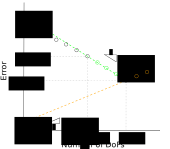
\includegraphics[width=0.5\linewidth]{../3_figure_plot/7_error_evolution_one_p/sketch_error_one_p.pdf}
     \caption{Conceptual sketch of the error against the number of $\text{DoFs}$.}
     \label{sketch_error_one_p}
 \end{figure}

\subsection{Implementation process}           \label{section_strategy}

When $E_h$ starts to decrease at the analytical rate, for which $E_h$ and $N_h$ read ${E_{\rm c}}$ and ${N_{\rm c}}$, respectively, $\alpha_{\rm T}$ can be inverted by using
\begin{equation}
 \alpha_{\rm T} = {E_{\rm c}}/{N_{\rm c}}^{- \beta_{\rm T}}.		\label{formula_offset_truncation_error}
\end{equation}
After this point, both the development of $E_{\rm T}$ and $E_{\rm R}$ are known. Obviously, $N_{\rm opt}$ occurs when $E_{\rm T}+E_{\rm R}$ is the smallest. By solving
\begin{equation}
    \frac{d(E_{\rm T}+E_{\rm R})}{dN}=0,    \label{derivative_condition_N_opt}
\end{equation}
we can predict
\begin{subequations}
\begin{align}
 N_{\rm opt} = \left( \frac{\alpha_{\rm T} \beta_{\rm T}}{\alpha _{\rm R} \beta_{\rm R}} \right)^{\frac{1}{\beta_{\rm T} + \beta_{\rm R}}},
\end{align}
and hence, the highest attainable accuracy
\begin{align}
 E_{\rm min} = \alpha_{\rm T} {N_{\rm opt}}^{- {\beta _{\rm T}}}+\alpha_{\rm R} {N_{\rm opt}}^{{\beta _{\rm R}}}.
\end{align}
\end{subequations}

\section{Determination of the error constants in Fig.~\ref{sketch_error_one_p}}  	\label{section_error_constants}

To determine the constants $\alpha_{\rm R}$ and $\beta_{\rm R}$ in Fig.~\ref{sketch_error_one_p}, we investigate three benchmark equations using various element degrees, followed by a wide range of second-order differential equations using one particular element degree. Furthermore, we analyse the influence of the solution strategy and boundary condition focusing on one element degree.

\subsection{Benchmark equations}

The benchmark equations are shown in Table~\ref{benchmark_equations}, for which the element degree ranges from 1 to 5.
The values of $\alpha_{\rm R}$ are shown in Fig.~\ref{py_offset_summary_bench}, which are as expected when using the double precision\cite{Alglib_custom}. The values of $\beta_{\rm R}$ are 2 using the standard FEM and 1 using the mixed FEM, which will be taken as constants if not stated otherwise. Note that, $\alpha_{\rm R}$ and $\beta_{\rm R}$ for one particular variable are basically the same for all the element degrees. 
                                                
\begin{table}[!ht]
\caption [sss] {Benchmark equations.}		% \footnotemark
\label{benchmark_equations} 
\centering
 \begin{tabular}{|C{2.5cm}|C{4.2cm}|C{3.8cm}|C{4cm}|} \hline   
{} & {Poisson} & {diffusion} & {Helmholtz} \\ \hline
{$d(x)$} & {$1$} & $1+x$ & $(1+i) e^{-x}$  \\	\hline
{$r(x)$} & {0} & 0 & $2 e^{-x}$ \\	\hline
{$f(x)$} & {$-e^{- (x-1/2)^2} \left({4x^2 - 4x -1} \right)$}  & $-2 \pi \cos (2 \pi x) + 4 {\pi}^2 \sin (2 \pi x)(x+1)$ & 0 \\ \hline
{$\|f(x)\|_2$} & {1.60} & {42.99} & {0.00} \\	\hline
\multirow{2}{2cm}{\centering Boundary conditions} & {$u(0) = e^{-1/4}$} & $u(0)=0$& $u (0) = 1$ \\	\cline{2-4}
&$u(1) = e^{-1/4}$ & $u_x(1)=2 \pi$  &$ u_x(1) = 0$ \\	\hline
Analytical solution $u(x)$ & {$e^{- (x-1/2)^2}$} & $\sin (2 \pi x)$ & $a e^{(1+i) x} + (1-a) e^{-i x}$, $a=1/{((1-i) e^{1+2i}+1)}$ \\	\hline
{$\|u(x)\|_2$} & {0.92} & 0.71 & 1.26 \\	\hline
\end{tabular}
\end{table}


\begin{figure}[!ht]
	\centering
    \begin{subfigure}{6.0cm}
        \includegraphics[width=1.0\linewidth]{../3_figure_plot/2_offset_summary/py_offset_summary_bench_sm.pdf}
        \caption{The standard FEM}
        \label{py_offset_summary_bench_sm}
    \end{subfigure}
    \hspace{-0.2cm}
    \begin{subfigure}{6.0cm}
        \includegraphics[width=1.0\linewidth]{../3_figure_plot/2_offset_summary/py_offset_summary_bench_mm.pdf}
        \caption{The mixed FEM}
        \label{py_offset_summary_bench_mm}
    \end{subfigure}
\caption{$\alpha_{\rm R}$ for the the benchmark equations.}
\label{py_offset_summary_bench}
\end{figure}

In addition, the theoretical order of convergence $\beta_{\rm T}$ can be reached fast as that shown in Fig.~\ref{sketch_error_one_p}. For the Poisson equation, the development of the order of convergence is shown in Table~\ref{evolution_convergence_order_sample_equations} when the approximation order is 3.

\newpage
\begin{table}[!ht]
\caption[sss]{An example for the evolution of the order of convergence.}
\label{evolution_convergence_order_sample_equations}
\hspace{3.5cm}
\begin{subtable}{0.4\textwidth}
\caption{The standard FEM}
 \begin{tabular}{c c c c} \hline
\multirow{2}{*}{} & \multicolumn{3}{c}{Refinement level} \\ \cline{2-4}
 & 2 & 3 & 4 \\	\hline
$u$ & 3.97 & 3.99 & 4.00 \\ 
$u_x$ & 4.02 & 4.00 & 4.00 \\ 
$u_{xx}$ & 3.87 & 3.98 & 4.00 \\ \hline
\end{tabular}
\end{subtable}
\hspace{-1.5cm}
\begin{subtable}{.4\textwidth}
\caption{The mixed FEM}
\begin{tabular}{c c c c} \hline
\multirow{2}{*}{} & \multicolumn{3}{c}{Refinement level} \\ \cline{2-4}
 & 2 & 3 & 4 \\	\hline
$u$ & 3.96 & 3.99 & 4.00 \\ 
$v$ & 4.02 & 4.00 & 4.00 \\ 
$v_{x}$ & 3.86 & 3.98 & 4.00 \\ \hline
\end{tabular}
\end{subtable}
\end{table}

\subsection{Wide range of second-order differential equations}	    \label{section_scaling}

First, to cover a wide range of $\|u\|_2$, together with $\|f\|_2$, for the Poisson equation, we investigate the cases shown in Table \ref{scaling_cases_Poisson}, for which the distribution of $\|u\|_2$ and $\|f\|_2$ can be found in Fig.~\ref{l2_norm_u_f} for Cases 1--4. Second, we investigate various $d(x)$ shown in Table~\ref{d_diffusion_equations} for the diffusion equations with $u=e^{-{(x-1/2)^2}}$. Last, we consider $r(x)$ from the first five cases of $d(x)$ in Table~\ref{d_diffusion_equations} for the Helmholtz equations with $u=e^{-{(x-1/2)^2}}$ and $d(x)=1$. Specifically, we restrict ourselves to $P_2$ and $P_4/P_3^{\rm disc}$ elements, and only Dirichlet boundary conditions are considered. 

\begin{table}[!ht]
\centering
\caption [w]{Settings of the Poisson equations with various $\|u\|_2$ and $\|f\|_2$.} 
\label{scaling_cases_Poisson}
 \begin{tabular}{c l l l} \hline      
Case & $f(x,c)$ & $u(x,c)$ & $c$ \\ \hline
1 & $\sin (2 \pi cx)$ & ${(2 \pi c)}^{-2} \sin (2 \pi cx)$ & \multirow{2}{*}{1e-2, 1e-1, 1e0, 1e1, 1e2} \\ \cline{1-3}
2 & $(2 \pi c) \sin (2 \pi c x)$ & ${(2 \pi c)}^{-1} \sin (2 \pi cx)$ &  \\ \hline
3 & $\sin (2 \pi c x) +1$ & ${(2 \pi c)}^{-2}\sin (2 \pi c x)-\frac{x^2}{2}$ & \multirow{4}{*}{1e-4, 1e-2, 1e0, 1e2, 1e4} \\ \cline{1-3}
4 & $\makecell{-e^{-{c}{(x-1/2)^2}} \cdot \\ \left({4{c}^2(x-1/2)^2 -2c} \right)}$ & $e^{-{c}{{(x-1/2)^2}}}$ &  \\ \cline{1-3}
5 & $0$ & ${c}^{-1} x$ &  \\ \hline
\end{tabular}
\end{table}

\begin{figure}[!ht]
\centering
    \includegraphics[width=0.42\linewidth]{../3_figure_plot/3_l2_norm_u_f/l2_norm_u_f.pdf}
    \caption{Distribution of $\|u\|_2$ and $\|f\|_2$ for the Poisson equations in Table~\ref{scaling_cases_Poisson}.}
    \label{l2_norm_u_f}
\end{figure}

\begin{table}[!ht]
\centering
\caption [w]{Various $d(x)$ for the diffusion equations.} 
\label{d_diffusion_equations}
 \begin{tabular}{c c c c c c} \hline
$\#$ &$d(x)$ & $\|d(x)\|_2$ & $\#$ &$d(x)$ & $\|d(x)\|_2$ \\ \hline
1 & 0.01 & 0.01 & 7 & $1+\sin(10x)$ & 1.14 \\ \hline
2 & 0.1 & 0.1 & 8 & $1+\sin(100x)$ & 1.06 \\ \hline
3 & 1 & 1 & 9 & $1+x$ & 1.5 \\ \hline
4 & 10 & 10 & 10 & $1+10x$ & 6.7 \\ \hline
5 & 100 & 100 & 11& $1+100x$ & 58.6 \\ \hline
6 & $1+\sin(x)$ & 1.23 & & &  \\ \hline
\end{tabular}
\end{table}

%\newpage

For the three types of equations, $\alpha_{\rm R}$ for different unknowns are shown in Fig.~\ref{py_offset_summary_Pois} -- Fig.~\ref{py_offset_summary_Helm}. Note that, the variable in the $x$ axis is $\|u\|_2$ for $u$ and $v$, and $\|v\|_2$ for $v_x$ in Fig.~\ref{py_offset_summary_Pois_mm}.

%\newpage
\begin{figure}[!ht]
	\centering
    \begin{subfigure}{6.0cm}
        \includegraphics[width=1.0\linewidth]{../3_figure_plot/2_offset_summary/py_offset_summary_Pois_sm.pdf}
        \caption{The standard FEM}
        \label{py_offset_summary_Pois_sm}
    \end{subfigure}
    \hspace{-0.2cm}
    \begin{subfigure}{6.0cm}
        \includegraphics[width=1.0\linewidth]{../3_figure_plot/2_offset_summary/py_offset_summary_Pois_mm.pdf}
        \caption{The mixed FEM}
        \label{py_offset_summary_Pois_mm}
    \end{subfigure}
\caption{$\alpha_{\rm R}$ for the Poisson equations in Table~\ref{scaling_cases_Poisson}.}
\label{py_offset_summary_Pois}
\end{figure}

\begin{figure}[!ht]
	\centering
    \begin{subfigure}{6.0cm}
        \includegraphics[width=1.0\linewidth]{../3_figure_plot/2_offset_summary/py_offset_summary_diff_sm.pdf}
        \caption{The standard FEM}
        \label{py_offset_summary_diff_sm}
    \end{subfigure}
    \hspace{-0.2cm}
    \begin{subfigure}{6.0cm}
        \includegraphics[width=1.0\linewidth]{../3_figure_plot/2_offset_summary/py_offset_summary_diff_mm.pdf}
        \caption{The mixed FEM}
        \label{py_offset_summary_diff_mm}
    \end{subfigure}
\caption{$\alpha_{\rm R}$ for the diffusion equations with $u=e^{-{(x-1/2)^2}}$ and various $\|d\|_2$ in Table~\ref{d_diffusion_equations}.}
\label{py_offset_summary_diff}
\end{figure}

\begin{figure}[!ht]
	\centering
    \begin{subfigure}{6.0cm}
        \includegraphics[width=1.0\linewidth]{../3_figure_plot/2_offset_summary/py_offset_summary_Helm_sm.pdf}
        \caption{The standard FEM}
        \label{py_offset_summary_Helm_sm}
    \end{subfigure}
    \hspace{-0.2cm}
    \begin{subfigure}{6.0cm}
        \includegraphics[width=1.0\linewidth]{../3_figure_plot/2_offset_summary/py_offset_summary_Helm_mm.pdf}
        \caption{The mixed FEM}
        \label{py_offset_summary_Helm_mm}
    \end{subfigure}
\caption{$\alpha_{\rm R}$ for the Helmholtz equations with $u=e^{-{(x-1/2)^2}}$, $\|d\|_2=1$ and $r(x)$ taken from the first five cases of $d(x)$ in Table~\ref{d_diffusion_equations}.}
\label{py_offset_summary_Helm}
\end{figure}

For the Poisson equations, $\alpha_{\rm R}$ is linearly proportional to the variable in the $x$ axis, for which the ratios are 2e-17, 5e-17 and 5e-16 for $u$, $u_x$ and $u_{xx}$ respectively using the standard FEM, and 1e-18, 1e-16 and 5e-16 for $u$, $v$ and $v_{x}$ respectively using the mixed FEM. To make $\alpha_{\rm R}$ independent of the unknowns, we propose the scaling schemes shown in Table~\ref{scaling_schemes_std_and_mix_FEM}, which allow us to recover the above constants irrespective of the magnitude of the unknowns. Note that, two schemes are needed for the mixed FEM: $M_1$ for $u$ and $v_x$, and $M_2$ for $v_x$.

\begin{table}[!ht]
\centering
\caption [sss] {System of equations using various scaling schemes.}
\label{scaling_schemes_std_and_mix_FEM} 
\begin{tabular}{c c c c}
\hline  
{Scheme}& Left-hand side & Solution & Right-hand side \\	\hline
$S$ & {$A$} & $\frac{1}{\|u\|_{2}} U$ & $\frac{1}{\|u\|_{2}} F$ \\	\hline
$M_1$ & {$\left[ \begin{array}{cc} M & \frac{\|u\|_{2}}{\|v\|_{2}} B  \\ B^T & 0 \end{array}\right]$ } & $\left[ \begin{array}{cc} \frac{1}{\|v\|_{2}} {V} \\ \frac{1}{\|u\|_{2}} {U} \end{array}\right]$ & $\frac{1}{\|v\|_{2}}\left[ \begin{array}{cc} G \\ { H} \end{array}\right]$\\	\hline
$M_2$ & {$\left[ \begin{array}{cc} M & B  \\ B^T & 0 \end{array}\right]$ } & $\frac{1}{\|u\|_{2}} \left[ \begin{array}{cc} {V} \\ {U} \end{array}\right]$ & $\frac{1}{\|u\|_{2}} \left[ \begin{array}{cc}  G \\ H \end{array}\right]$ \\	\hline
\end{tabular}
\end{table}


For the diffusion equations, $\alpha_{\rm R}$ is linearly proportional to $\|d(x)\|_2$ for $v$ and $v_x$ using the mixed FEM, for which the ratios are 2e-16 and 5e-16, respectively, while it is relatively independent of $d(x)$ in other scenarios. For the Helmholtz equations, $\alpha_{\rm R}$ is independent of $r(x)$.

\newpage
In summary, by using the scaling schemes in Table~\ref{scaling_schemes_std_and_mix_FEM}, we obtain $\alpha_{\rm R}$ in Table~\ref{relation_alpha_R_l2_norm_u_du} that are independent of the unknowns. Note that, these numbers are also valid for the benchmark equations.

\begin{table}[!ht]
\captionof{table}{Variable-independent $\alpha_{\rm R}$ for the second-order differential equations.}
\hspace{4.0cm}
\begin{subtable}{0.4\textwidth}
\caption{The standard FEM}
\begin{tabular}{l l}
\hline
$u$ & 2e-17 \\ \hline 
$u_x$ & 5e-17 \\ \hline
$u_{xx}$ & 1e-15 \\ \hline
\end{tabular}
\end{subtable}
\hspace{-2.5cm}
\begin{subtable}{.4\textwidth}
\caption{The mixed FEM}
\begin{tabular}{l l l l}
\hline
$u$ & 5e-17 \\ \hline 
$v$ & 2e-16 $\times \|d(x)\|_2$ \\ \hline
$v_x$ & 5e-16 \\ \hline
\end{tabular}
\end{subtable}
\label{relation_alpha_R_l2_norm_u_du}
\end{table}


\newpage
\subsection{Sensitivity analysis}       \label{section_sensitivity}

We focus on the benchmark Poisson equation.

%\newpage

\subsubsection{Boundary conditions}	\label{section_BC}

We consider two aspects for the influence of boundary conditions: the type of boundary conditions and the weak imposition of the Dirichlet boundary condition using the standard FEM.

For the first part, the Dirichlet boundary condition at the left boundary ($x=0$) is kept while that at the right boundary ($x=1$) has been replaced by the Neumann boundary condition $u_x (1) = -e^{-1/4}$, leading to the same solution and derivative profiles. 
For the standard FEM with $P_2$ elements, using the Dirichlet/Neumann boundary condition, the offset $\alpha_{\rm R}$ is slightly larger than that using the Dirichlet/Dirichlet boundary condition for $u$ and $u_x$, by a factor of 3.5 and 2 respectively; $\alpha_{\rm R}$ is equal to that using the Dirichlet/Dirichlet boundary condition for $u_{xx}$. For the mixed FEM with $P_4/P_3^{\rm disc}$ elements, using the Dirichlet/Neumann boundary condition, $\alpha_{\rm R}$ increases to 3e-17 for $u$, is 5 times smaller for $v$, and does not change for $v_x$.

For the second part, the weak imposition of the Dirichlet boundary condition produces the same error when the penalty parameter is large enough, e.g. $10^6$.

In summary, the boundary condition basically makes no difference to the values of $\alpha_{\rm R}$ we proposed in Table~\ref{relation_alpha_R_l2_norm_u_du}.

\subsubsection{Solution strategy}		\label{section_solver}

The alternative solution method to the UMFPACK solver is the iterative Conjugate Gradient (CG) method\cite{ginsburg1963cg}, which can be applied when the left-hand side is symmetric and positive definite. We focus on the tolerance of the CG solver, denoted by $tol_{prm}$: the iteration stops when the norm of the residual is smaller than it.

For the standard FEM, the CG method can be applied directly. However, for the mixed FEM, since the left-hand side of Eq.~(\ref{matrix equation mix FEM}) is indefinite, this method is used after segregating Eq.~(\ref{matrix equation mix FEM}) based on the Schur complement, which results in
\begin{subequations}
 \begin{align}
  B^{\top} M^{-1} B U &= B^{\top} M^{-1} G - H, 	\label{schur_complement_solution} \\
  MV&=G-BU.						\label{schur_complement_gradient}
\end{align}						\label{schur_complement_solu_grad}%
\end{subequations}
In the solution process of Eq.~(\ref{schur_complement_solu_grad}), the CG solver can be used for the left-hand side being either $B^{\top}M^{-1}B$ (Schur complement) or $M$. In particular, we investigate the former while the UMFPACK solver is used for the left-hand side being $M$.  

Focusing on $u$ with the approximation order of 3, the evolution of the error for various $tol_{prm}$ using the CG solver is illustrated in Fig.~\ref{py_bench_Pois_error_solution_strategy}, in comparison with that using the UMFPACK solver.
It shows that the CG solver introduces iteration errors when $tol_{prm}$ is less strict.
Specially, for the mixed FEM, the accuracy using the CG solver can not be as high as that using the UMFPACK solver. This proves the correctness of choosing the UMFPACK solver to obtain higher accuracy. 

\begin{figure}[!ht]
	\centering
    \begin{subfigure}{6.0cm}
        \includegraphics[width=1.0\linewidth]{../3_figure_plot/4_solution_strategy/py_error_comparison_solution_strategy_SM_solu.pdf}
        \caption{The standard FEM}
        \label{py_bench_Pois_SM_error_solution_strategy_solu}
    \end{subfigure}
    \hspace{-0.2cm}
    \begin{subfigure}{6.0cm}	                		 	
        \includegraphics[width=1.0\linewidth]{../3_figure_plot/4_solution_strategy/py_error_comparison_solution_strategy_MM_solu.pdf}
        \caption{The mixed FEM}
        \label{py_bench_Pois_MM_error_solution_strategy_solu}
    \end{subfigure}
\caption{Comparison of the errors using the CG solver and the UMFPACK solver for $u$.}
\label{py_bench_Pois_error_solution_strategy}
\end{figure}



\section{Algorithm and its application}		\label{section_algorithm_application}

Based on the approach given in section \ref{approach_finding_optimal_number_of_DoFs}, and scaling schemes and error constants provided in section \ref{section_error_constants}, we introduce a practical algorithm and apply it to a complex-valued Helmholtz equation.

\subsection{Algorithm}

In this algorithm, we define the following coefficients and use them in the steps given below.

\begin{itemize}
  \renewcommand\labelitemi{--}
  \item a minimal number of $h$-refinements as a precondition, denoted by $R_{\rm min}$, with the following default values:
  \begin{equation}
  \begin{aligned}
      R_{\rm min} &=
      \begin{cases*}
	9-p & for p $<$ 6, \\
	4 & otherwise.
      \end{cases*}
  \end{aligned}
  \end{equation} 
  \item the allowed maximum $N_h$ : $10^8$, denoted by $N_{\rm max}$.  
  \item a stopping criterion $c_s$ for seeking the scaling factor $\|var\|_{2}$ in Table~\ref{scaling_schemes_std_and_mix_FEM}, which is 0.001 by default.
  \item a relaxation coefficient $c_r$ for seeking the theoretical order of convergence, with the following default values: 
    \begin{equation}
    \begin{aligned}
	c_r &=
	\begin{cases*}
	  0.9 & for p $<$ 4, \\
	  0.7 & for 4 $\leqslant$ p $<$ 10, \\
	  0.5 & otherwise.
	\end{cases*}
    \end{aligned}
    \end{equation}    
\end{itemize}

\paragraph{Step-1} `\textit{INPUT}'. In this step, the custom input shown in Table~\ref{settings_algorithm} has to be provided.

\begin{table}[!ht]
\captionof{table}{Custom input of the algorithm.}
\label{settings_algorithm}
  \centering
  \begin{tabular}{l L{10cm}}
    \toprule
    Type & Item  \\
    \midrule
    Problem & \tabitem the differential equation to be solved \\
     		& \tabitem variables of interest \\ \hline
    FEM     & \tabitem standard or mixed formulation \\
    		& \tabitem an ordered array of element degrees $\{p_{\min}, \ldots, p_{\rm max}\}$ \\
    \bottomrule
  \end{tabular}
\end{table}

\paragraph{Step-2} `\textit{NORMALIZATION}'. This step is used to find the scaling factors to normalize the variable of interest since the scaling factors do not exist for most practical problems. The specific procedure can be found in Algorithm \ref{algo_scaling_factor}.

\vspace{0.2cm}
\begin{algorithm}[H]
\caption{NORMALIZATION}
\label{algo_scaling_factor}
\While{$N_h<N_{\rm max}$}
{
    \eIf{$\left|\frac{\|var_{h}\|_{2} - \|var_{2h}\|_{2}}{\|var_{h}\|_{2}} \right| < c_s$}
    {
        $\|var\|_{2}$ $\gets$ $\|var_{h}\|_{2}$\;
        break\;
    }
    {
        $h$ $\gets$ $h/2$\;
        calculate $\|var_h\|_{2}$\;    
    }
}
\end{algorithm}
                                                                   
\paragraph{Step-3} `\textit{PREDICTION}'. This step illustrates how to find $E_{\rm min}$ based on the order of convergence.
The procedure for carrying out this step can be found in Algorithm \ref{block_PREDICTION}.

\vspace{0.2cm}
\begin{algorithm}[H]
\caption{PREDICTION}			% Seeking the analytical order of convergence Predicting $N_{\rm opt}$ and $E_{\rm min}$
\label{block_PREDICTION}
    \While{$\widetilde {E_{h}}>E_{\rm R}$ \textbf{\textup{and}} $N_h<N_{\rm max}$}
    {
        $\widetilde{Q}$ $\gets$ $\log _2 \left( {\widetilde {E_{2h}}}/{\widetilde {E_{h}}} \right)$\;
        \eIf
        {
            $\widetilde{Q} \geqslant \beta_{\rm T} \times c_r$
        }
        {
            $N_{\rm c} \gets N_h$\;
            $E_{\rm c} \gets \widetilde {E_{h}}$\;
            $\alpha_{\rm T}$ $\gets$ ${E_{\rm c}}/{N_{\rm c}}^{- \beta_{\rm T}}$\;
            $N_{\rm opt} \gets \left( \frac{\alpha_{\rm T} \beta_{\rm T}}{\alpha _{\rm R} \beta_{\rm R}} \right)^{\frac{1}{\beta_{\rm R} + \beta_{\rm T}}}$\;
            $E_{\rm min} \gets \alpha_{\rm T} {N_{\rm opt}}^{- {\beta _{\rm T}}} + \alpha_{\rm R} {N_{\rm opt}}^{{\beta _{\rm R}}}$\;

        }
        {
            $h$ $\gets$ $h/2$\;
            calculate $\widetilde {E_{h}}$ using Eq.~(\ref{formula_abs_error_numerical}) with proper scaling schemes\;
        }
	}    
\end{algorithm}

\paragraph{Step-4} `\textit{OUTPUT}'. In this step, we output $E_{\rm min}$ obtained from $Step$-3.

\subsection{Application}		\label{section_validation}

The problem reads\citep{chernetsky2010effect}:
\begin{equation}
  \left((0.01+x)(1.01-x) u_x \right)_x -(0.01i) u(x) = 1.0,\qquad x \in I = (0,1),	\label{1D_Helmholtz_equation_application}
\end{equation}
with boundary conditions imposed as follows: $u(0)=0$ and $u_x(1)=0$.

For the element degree $p$ being $\{1, 2, \ldots, 5\}$ using both the standard and mixed FEMs, $E_{\rm min}$ predicted by the algorithm are given in Fig.~\ref{E_min_application}. They fits that using the brute-force approach well.
However, the CPU time is saved much using the algorithm, see Fig.~\ref{CPU_application} for the CPU time used and Fig.~\ref{CPU_percentage_application} for the percentage of CPU time saved using the algorithm. Basically, the CPU time can be saved more than 60\% and 40\% for the standard FEM and the mixed FEM, respectively.

\begin{figure}[!ht]
	\centering
    \begin{subfigure}{6.0cm}
        \includegraphics[width=1.0\linewidth]{../3_figure_plot/6_comparison_brute-force_prediction/py_comparison_dofinder_accuracy_sm.pdf}
        \caption{The standard FEM}
        \label{E_min_application_sm}
    \end{subfigure}
    \hspace{0.0cm}
    \begin{subfigure}{6.0cm}	                		 	
        \includegraphics[width=1.0\linewidth]{../3_figure_plot/6_comparison_brute-force_prediction/py_comparison_dofinder_accuracy_mm.pdf}
        \caption{The mixed FEM}
        \label{E_min_application_mm}
    \end{subfigure}
\caption{$E_{\rm min}$ for Eq. (\ref{1D_Helmholtz_equation_application}) using the algorithm. The filled circle denotes results using the brute-force refinement.}
\label{E_min_application}
\end{figure}

\begin{figure}[!ht]
	\centering
    \begin{subfigure}{6.0cm}
        \includegraphics[width=1.0\linewidth]{../3_figure_plot/6_comparison_brute-force_prediction/py_comparison_dofinder_cpu_sm.pdf}
        \caption{The standard FEM}
        \label{CPU_application_sm}
    \end{subfigure}
    \hspace{0.0cm}
    \begin{subfigure}{6.0cm}	                		 	
        \includegraphics[width=1.0\linewidth]{../3_figure_plot/6_comparison_brute-force_prediction/py_comparison_dofinder_cpu_mm.pdf}
        \caption{The mixed FEM}
        \label{CPU_application_mm}
    \end{subfigure}
\caption{CPU time used to obtain $E_{\rm min}$ for Eq. (\ref{1D_Helmholtz_equation_application}) using the algorithm.}
\label{CPU_application}
\end{figure}

\begin{figure}[!ht]
	\centering
    \begin{subfigure}{6.0cm}
        \includegraphics[width=1.0\linewidth]{../3_figure_plot/6_comparison_brute-force_prediction/py_comparison_dofinder_percentage_cpu_sm.pdf}
        \caption{The standard FEM}
        \label{CPU_percentage_application_sm}
    \end{subfigure}
    \hspace{0.0cm}
    \begin{subfigure}{6.0cm}	                		 	
        \includegraphics[width=1.0\linewidth]{../3_figure_plot/6_comparison_brute-force_prediction/py_comparison_dofinder_percentage_cpu_mm.pdf}
        \caption{The mixed FEM}
        \label{CPU_percentage_application_mm}
    \end{subfigure}
\caption{Percentage of CPU time saved to obtain $E_{\rm min}$ for Eq. (\ref{1D_Helmholtz_equation_application}) using the algorithm.}
\label{CPU_percentage_application}
\end{figure}


\section{Conclusions}		\label{paragraph on conclusion}

A novel approach is presented to predict the highest attainable accuracy for one-dimensional second-order ordinary differential equations using the finite element methods.
In contrast to the brute-force approach, which uses monolithic $h$-refinements, this approach uses only a few coarse grid refinements. 
This approach takes advantage of the properpty of the order of convergence and the bound for the round-off error, and it is viable for the solution and its first and second derivative, using both the standard FEM and the mixed FEM with different element degrees.
The algorithm for implementing the approach shows that the highest attainable accuracy can be accurately predicted and the CPU time is significantly reduced. To compute the solution of the highest attainable accuracy using our approach, the CPU time can be saved more than 60\% for the standard FEM and 40\% for the mixed FEM.

Future research will focus on the validation of the approach for two-dimensional second-order problems, where the influence of the linear system solver, local mesh refinement and boundary conditions might be significantly different from one-dimensional problems. 

\appendix

\section{Derivation of the weak form}		\label{weak form appendix}

\subsection{The standard FEM}		\label{derivation_weak_form_SM}

Multiply Eq. (\ref{1d_second_order_differential_equation}) by a test function $\eta \in H ^1 (I)$, and integrate it over $I$ yield
\begin{equation}
(\eta, \, -\left(d u_x \right)_x + ru) = (\eta, \, f). \label{1D_general_inte}
\end{equation}
By applying Gauss's theorem, we obtain
\begin{equation}
 ({\eta} _x, \, d u_x) + (\eta, \, ru) = (\eta, \, f) + \left( \eta, \, d u_x n \right)_{ {\Gamma_N}},		\label{1D_general_gauss}
\end{equation}
which gives that shown in Eq.~({\ref{1D_general_SM_weak_form_Diri_strong}}). Adding auxiliary terms to the above equation renders Eq. (\ref{1D_general_SM_weak_form_Diri_weak}).

\subsection{The mixed FEM}		\label{derivation_weak_form_MM}
As a first step, we introduce the auxiliary variable
\begin{subequations}
\begin{align}
   v(x) = - d(x)u_x, \label{Gene_MM_strong1} 
\end{align}  
allowing Eq. (\ref{1d_second_order_differential_equation}) to be rewritten as
\begin{align}
  -v_x - r(x)u(x) = -f(x).  \label{Gene_MM_strong2}
\end{align}	\label{1D_general_MM_2in1}%
\end{subequations}
Multifply Eq. (\ref{Gene_MM_strong1}) by a test function of $v$, i.e. $w \in H _{N0}^{1}(I)$, and integrate it over $I$ yield
\begin{subequations}
\begin{align}
  ( d^{-1}v + u _x, w) = 0.	\label{Gene_MM_weak1_a}
\end{align}
Applying Gauss's theorem to Eq.~(\ref{Gene_MM_weak1_a}), it becomes
\begin{align}
 (w, \, d^{-1}v) - (w_x, \,  u ) = -(w, \, g n)_{\Gamma_D}.		\label{Gene_MM_weak1_b}
\end{align}				\label{Gene_MM_weak1}%
\end{subequations}
Multiply Eq. (\ref{Gene_MM_strong2}) by a test function of $u$, i.e. $q \in L^2 (I)$, and integrate it over $I$ yield
\begin{align}
- ( q , \, v_x) + (q, \, ru) = (q, \, f ). \label{Gene_MM_weak2}
\end{align}
Eq.~(\ref{Gene_MM_weak1_b}) and Eq.~({\ref{Gene_MM_weak2}}) result in those shown in Eq. (\ref{1D_General_MM_weak_2in1}).

\bibliographystyle{unsrt}  
\bibliography{mybibfile}  %%% Remove comment to use the external .bib file (using bibtex). 3_writing/1_1d/


\end{document}
